\documentclass{article}
\usepackage[utf8]{inputenc}

\title{Assignment 3}
\author{Benny Chen}
\date{\today}

\usepackage{color}
\usepackage{amsthm}
\usepackage{amssymb} 
\usepackage{amsmath}
\usepackage{listings}
\usepackage{xcolor}
\usepackage{listings}
\usepackage{graphicx}
\usepackage{enumitem}
\usepackage[hidelinks]{hyperref}

\definecolor{codegreen}{rgb}{0,0.6,0}
\definecolor{codegray}{rgb}{0.5,0.5,0.5}
\definecolor{codepurple}{rgb}{0.58,0,0.82}
\definecolor{backcolour}{rgb}{0.95,0.95,0.92}

\lstdefinestyle{mystyle}{
    backgroundcolor=\color{backcolour},   
    commentstyle=\color{codegreen},
    keywordstyle=\color{magenta},
    numberstyle=\tiny\color{codegray},
    stringstyle=\color{codepurple},
    basicstyle=\ttfamily\footnotesize,
    breakatwhitespace=false,         
    breaklines=true,                 
    captionpos=b,                    
    keepspaces=true,                 
    numbers=left,                    
    numbersep=5pt,                  
    showspaces=false,                
    showstringspaces=false,
    showtabs=false,                  
    tabsize=2
}

\lstset{style=mystyle}

\begin{document}

\maketitle

\section{Kernels for SVM}

\subsection{}
In the lecture of Support Vector Machine, we have discussed the kernel function, which can map the data points into a new high-dimensional space.
\\
Let $k_1(x,y)$ and $k_2(x,y)$ be the \textit{valid kernels}, that is, each of these two kernel functions can be decomposed into the product of two feature mapping functions $\Phi (x), i.e, k_1(x,y) = \Phi_1 {(x)}^T \Phi_1 (y)$ and $k_2(x,y) = \Phi_2 {(x)}^T \Phi_2 (y)$.
\\
Please show that $k(x,y) = k_1(x,y) + k_2(x,y)$ is also a valid kernel function by decomposing it into product of two feature mapping functions.

\subsubsection*{Answer:}

\begin{align*}
    k(x,y) &= k_1(x,y) + k_2(x,y) \\
    &= \Phi_1 {(x)}^T \Phi_1 (y) + \Phi_2 {(x)}^T \Phi_2 (y) \\
    &= \begin{bmatrix}
        \Phi_1 {(x)}^T & \Phi_2 {(x)}^T
    \end{bmatrix}
    \begin{bmatrix}
        \Phi_1 (y) \\
        \Phi_2 (y)
    \end{bmatrix} \\
    &= \begin{bmatrix}
        \Phi_1 {(x)}^T & \Phi_2 {(x)}^T
    \end{bmatrix}
    \begin{bmatrix}
        \Phi_1 (y) \\
        0
    \end{bmatrix} +
    \begin{bmatrix}
        \Phi_1 {(x)}^T & \Phi_2 {(x)}^T
    \end{bmatrix}
    \begin{bmatrix}
        0 \\
        \Phi_2 (y)
    \end{bmatrix} \\
    &= \begin{bmatrix}
        \Phi_1 {(x)}^T & 0
    \end{bmatrix}
    \begin{bmatrix}
        \Phi_1 (y) \\
        0
    \end{bmatrix} +
    \begin{bmatrix}
        0 & \Phi_2 {(x)}^T
    \end{bmatrix}
    \begin{bmatrix}
        0 \\
        \Phi_2 (y)
    \end{bmatrix} \\
    &= \begin{bmatrix}
        \Phi_1 {(x)}^T & 0
    \end{bmatrix}
    \begin{bmatrix}
        \Phi_1 (y) \\
        0
    \end{bmatrix} +
    \begin{bmatrix}
        0 & \Phi_2 {(x)}^T
    \end{bmatrix}
    \begin{bmatrix}
        0 \\
        \Phi_2 (y)
    \end{bmatrix} \\
    &= \begin{bmatrix}
        \Phi_1 {(x)}^T &
        \Phi_2 {(x)}^T
    \end{bmatrix}
    \begin{bmatrix}
        \Phi_1 (y) \\
        \Phi_2 (y)
    \end{bmatrix} \\
    &= \Phi {(x)}^T \Phi (y)
\end{align*}

The product of two feature mapping functions is $\Phi {(x)}^T \Phi (y)$.


\section{K-Means and Cluster Validation}

\subsection{}

Consider the following set of one-dimensional points:
\begin{center}
    \{0.1, 0.2, 0.45, 0.55, 0.8, 0.9\}
\end{center}

All the points are located in the range between [0,1]. Suppose we apply k-means clustering to obtain three clusters, A, B, and C. If the initial centroids are located at {0, 0.4, 1}, respectively, please find:

\begin{enumerate}[label= (\alph*)]
    \item The cluster assignments (fill in either A, B, or C for each data point);
    \item Locations of the centroids (coordinate) after the first three iterations by filling out the following table.
\end{enumerate}

\subsubsection*{Answer:}

\begin{table}[ht]
    \centering
    \begin{tabular}{llllllllll}
    Iter & 0.10 & 0.25 & 0.45 & 0.55 & 0.80 & 0.90 & A & B & C \\
    0 & --- & --- & --- & --- & --- & --- & 0.00 & 0.40 & 1.00 \\
    1 & A  & A & B & B & C & C & 0.15 & 0.50 & 0.85 \\
    2 & A  & A & B & B & C & C & 0.15 & 0.50 & 0.85\\
    3 & A  & A & B & B & C & C & 0.15 & 0.50 & 0.85 
    \end{tabular}
\end{table}

\subsection{}
The following table shows the clustering results in a land cover classification dataset that consists of many pieces of land. The number provided in the table is the number of objects (pieces of land) that are clustered into each cluster that belongs to each category. For example, the number in the forest column and cluster 1 row means that 10 forest items are clustered into cluster 1.

\begin{table}[ht]
    \centering
    \begin{tabular}{llllll}
     & Forest & Farm & Shrubland & Urban & Water \\
    Cluster 1 & 20 & 10 & 10 & 10 & 950 \\
    Cluster 2 & 400 & 100 & 400 & 50 & 50 \\
    Cluster 3 & 50 & 50 & 500 & 200 & 200 \\
    Cluster 4 & 200 & 250 & 150 & 200 & 200
    \end{tabular}
\end{table}

Which cluster has the smallest entropy? Which cluster has the largest entropy?

\subsubsection*{Answer:}

\begin{enumerate}[label= (\alph*)]
    \item Cluster 1: $20 + 10 + 10 + 10 + 950 = 1000$
    \\
    Entropy:
    \begin{equation*}
        -\frac{20}{1000}\log_2(\frac{20}{1000}) - 3(\frac{10}{1000}\log_2(\frac{10}{1000})) - \frac{950}{1000}\log_2(\frac{950}{1000}) = 0.38249
    \end{equation*}
    \item Cluster 2: $400 + 100 + 400 + 50 + 50 = 1000$
    \\
    Entropy:
    \begin{equation*}
        -2(\frac{400}{1000}\log_2(\frac{400}{1000})) - 2(\frac{50}{1000}\log_2(\frac{50}{1000})) - \frac{100}{1000}\log_2(\frac{100}{1000}) = 1.82193
    \end{equation*}
    \item Cluster 3: $50 + 50 + 500 + 200 + 200 = 1000$
    \\
    Entropy:
    \begin{equation*}
        -2(\frac{50}{1000}\log_2(\frac{50}{1000})) - \frac{500}{1000}\log_2(\frac{500}{1000}) - 2(\frac{200}{1000}\log_2(\frac{200}{1000})) = 1.52193
    \end{equation*}
    \item Cluster 4: $200 + 250 + 150 + 200 + 200 = 1000$
    \\
    Entropy:
    \begin{equation*}
        -3(\frac{200}{1000}\log_2(\frac{200}{1000})) - \frac{250}{1000}\log_2(\frac{250}{1000}) - \frac{150}{1000}\log_2(\frac{150}{1000}) = 2.30370
    \end{equation*}
\end{enumerate}

Cluster 1 has the smallest entropy, and Cluster 4 has the largest entropy.

\subsection{}

Please provide True or False, followed by the Short Answer on your explanations.

\begin{enumerate}[label= (\alph*)]
    \item When clustering a dataset using K-means, whenever SSE decreases, cohesion increases.
    \item With the given initial centroid in the following diagram: When the k-means algorithm completes, each shaded circle will have one cluster centroid at its center.
    \begin{center}
        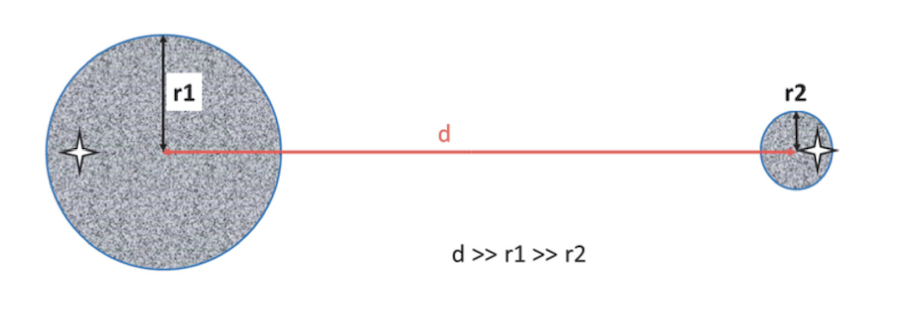
\includegraphics[scale=0.5]{images/Q2P3A.png}
    \end{center}
    \item With the given initial centroids: When the k-means algorithms completes, there will be one cluster centroid in the center of each of the two shaded regions, and each of the two final clusters will consist only of points from one of the shaded regions. In other words, none of the two final clusters will have points from both shaded regions.
    \begin{center}
        
\includegraphics[scale=0.5]{images/Q2P3B.png}
    \end{center}
\end{enumerate}

\subsubsection*{Answer:}

\begin{enumerate}[label= (\alph*)]
    \item True. 
    \item True.
    \item False.
\end{enumerate}

\subsection{}

The distance matrices (Euclidean distance) below (\textbf{Figures A, B, and C}) are sorted according to cluster labels, and correspond, in some order, to the sets of points (Figures D, E, and F).
\\
Differences in color distinguish between clusters, and each set of points contains 100 points and four clusters, each of equal size. In the distance matrix, blue indicates the smallest distances, and red indicates the largest distances.

\begin{enumerate}[label= (\alph*)]
    \item Match the distance matrices (\textbf{Figures A, B, and C}) with the right sets of points (\textbf{Figures D, E, and F}). Please note that the colors of the data points in Figures D-F DO NOT match the colors in the distance matrices in Figures A-C.
    \item For the symmetric matrix given in \textbf{Figure B}, match the four rows to the corresponding clusters (characterized by four colors --- red, blue, green, and magenta) in the dataset that you match with it in the previous question.
\end{enumerate}

\subsubsection*{Answer:}
\begin{enumerate}[label= (\alph*)]
    \item \begin{table}[ht]
        \centering
        \begin{tabular}{ll}
        Matrices & Datasets \\
        1(a) & F \\
        1(b) & D \\
        1(c) & E
        \end{tabular}
    \end{table}
    \item     \begin{table}[ht]
        \centering
        \begin{tabular}{ll}
        Matrix Rows   & Cluster (Represented by Colors) \\
        1st (1--100)   & Red \\
        2nd (101--200) & Green \\
        3rd (201--300) & Blue \\
        4th (301--400) & Magenta
        \end{tabular}
    \end{table}
\end{enumerate}

\begin{center}
    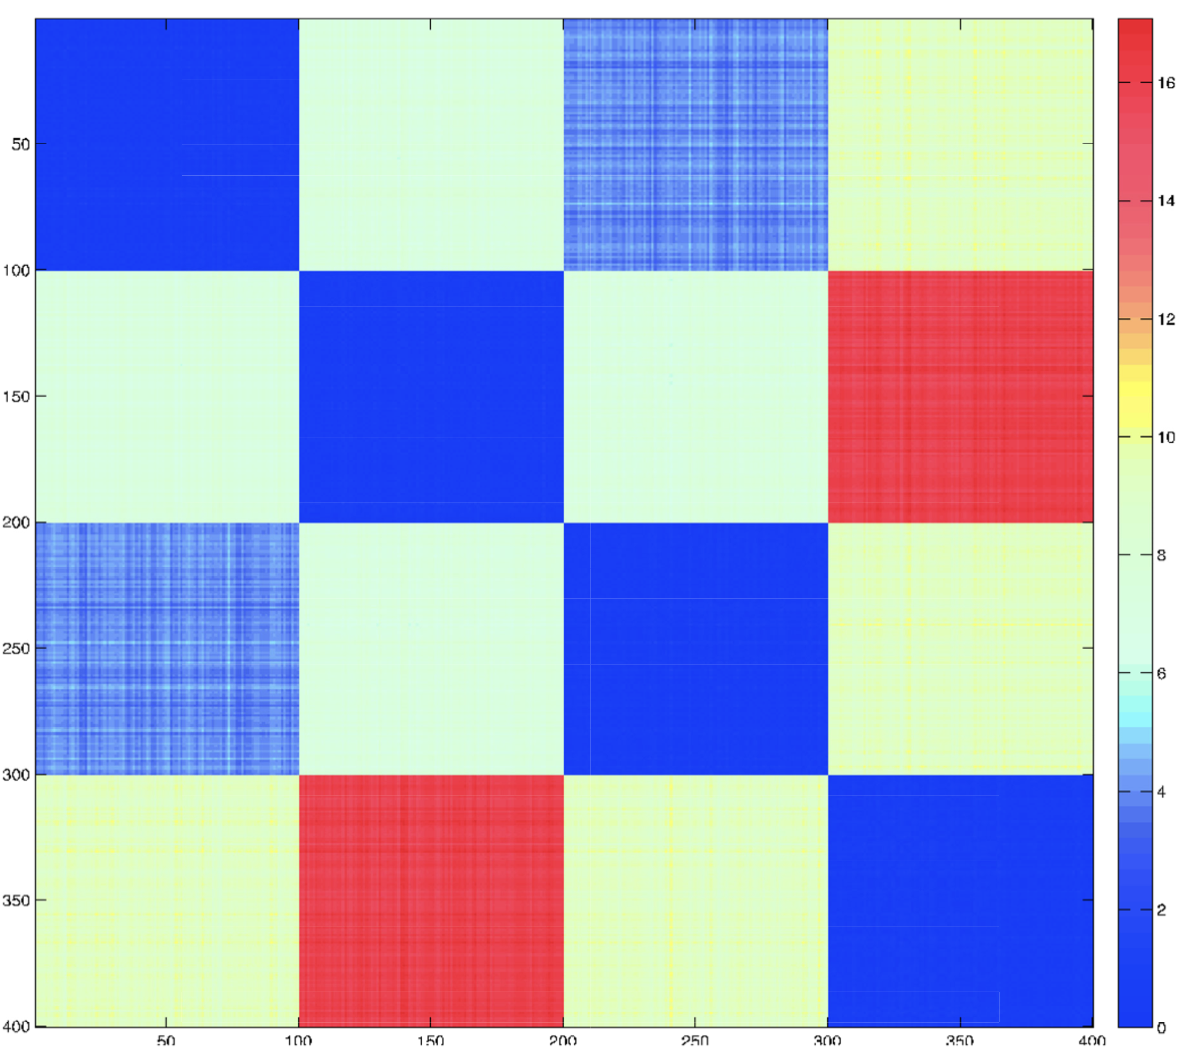
\includegraphics[scale=0.5]{images/Q2P4A.png}
\end{center}

\begin{center}
    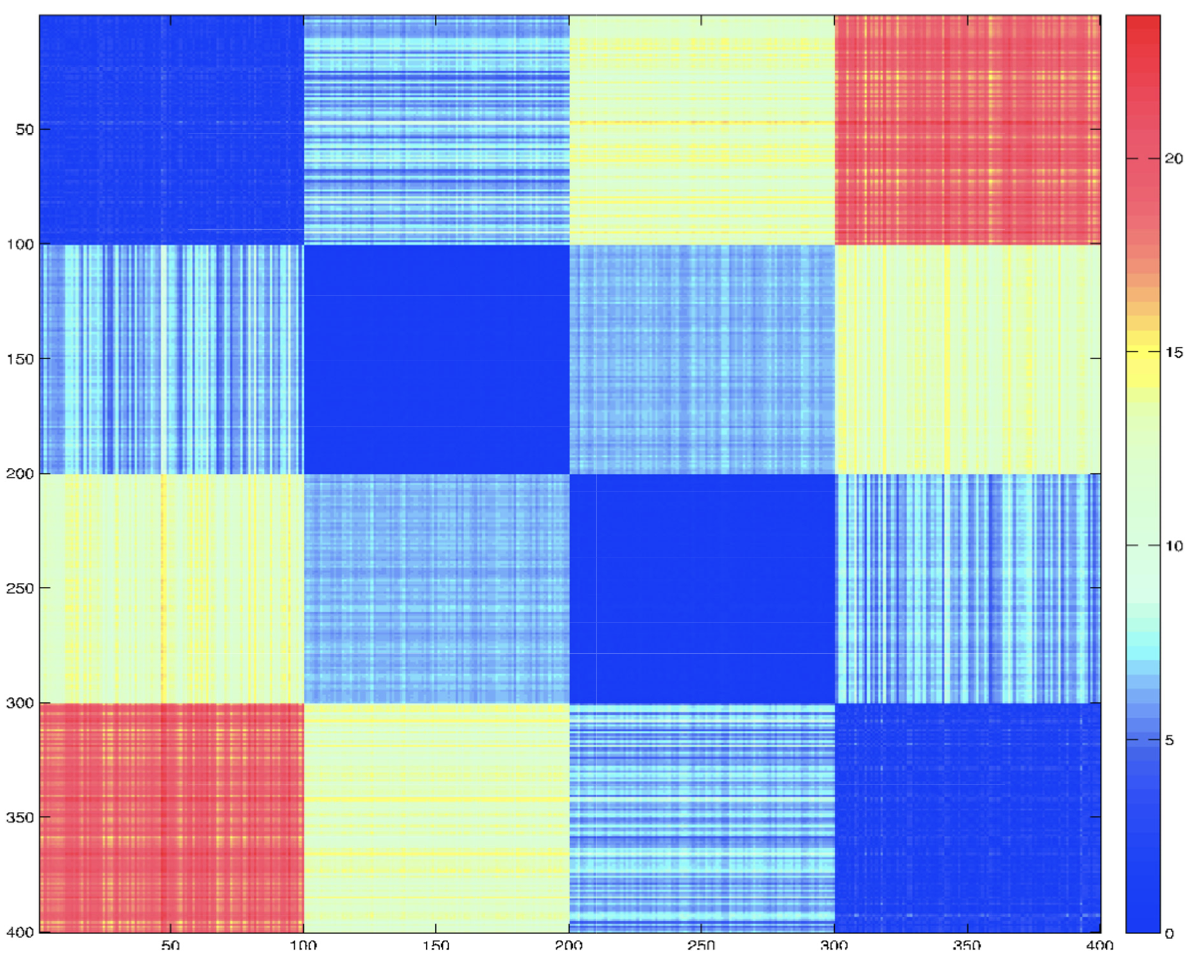
\includegraphics[scale=0.5]{images/Q2P4B.png}
\end{center}

\begin{center}
    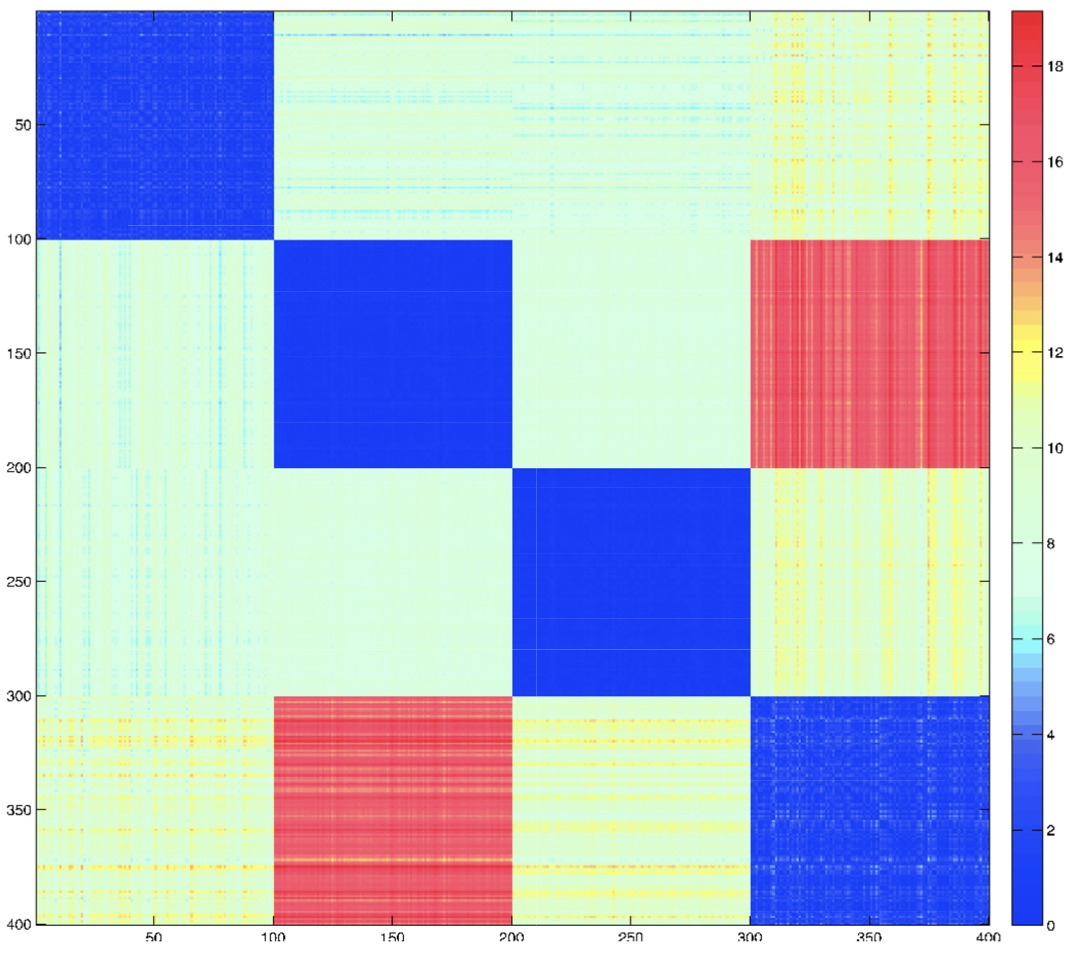
\includegraphics[scale=0.5]{images/Q2P4C.png}
\end{center}

\begin{center}
    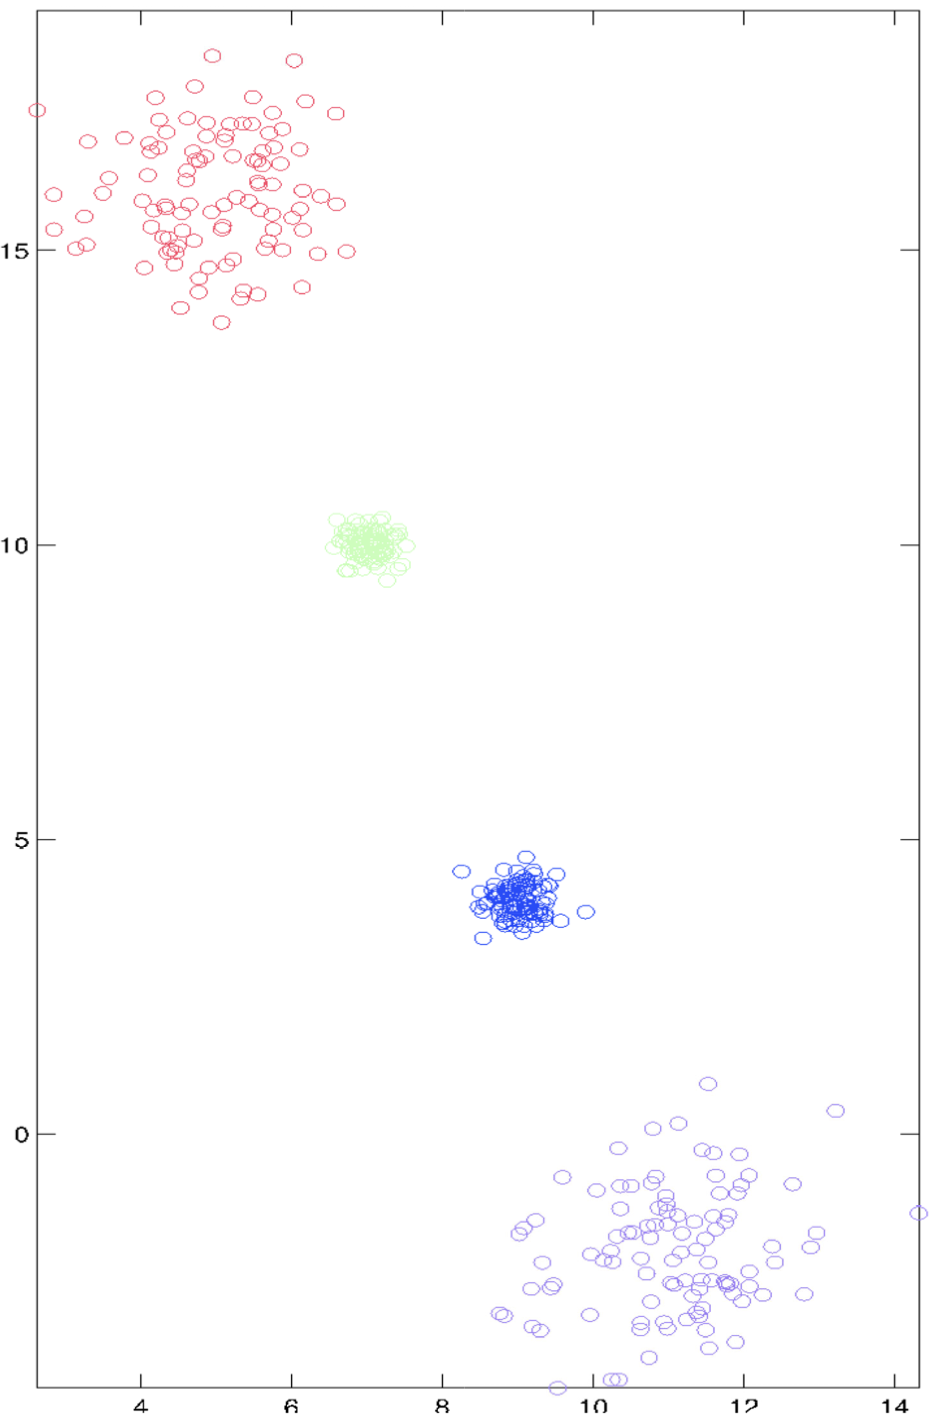
\includegraphics[scale=0.5]{images/Q2P4D.png}
\end{center}

\begin{center}
    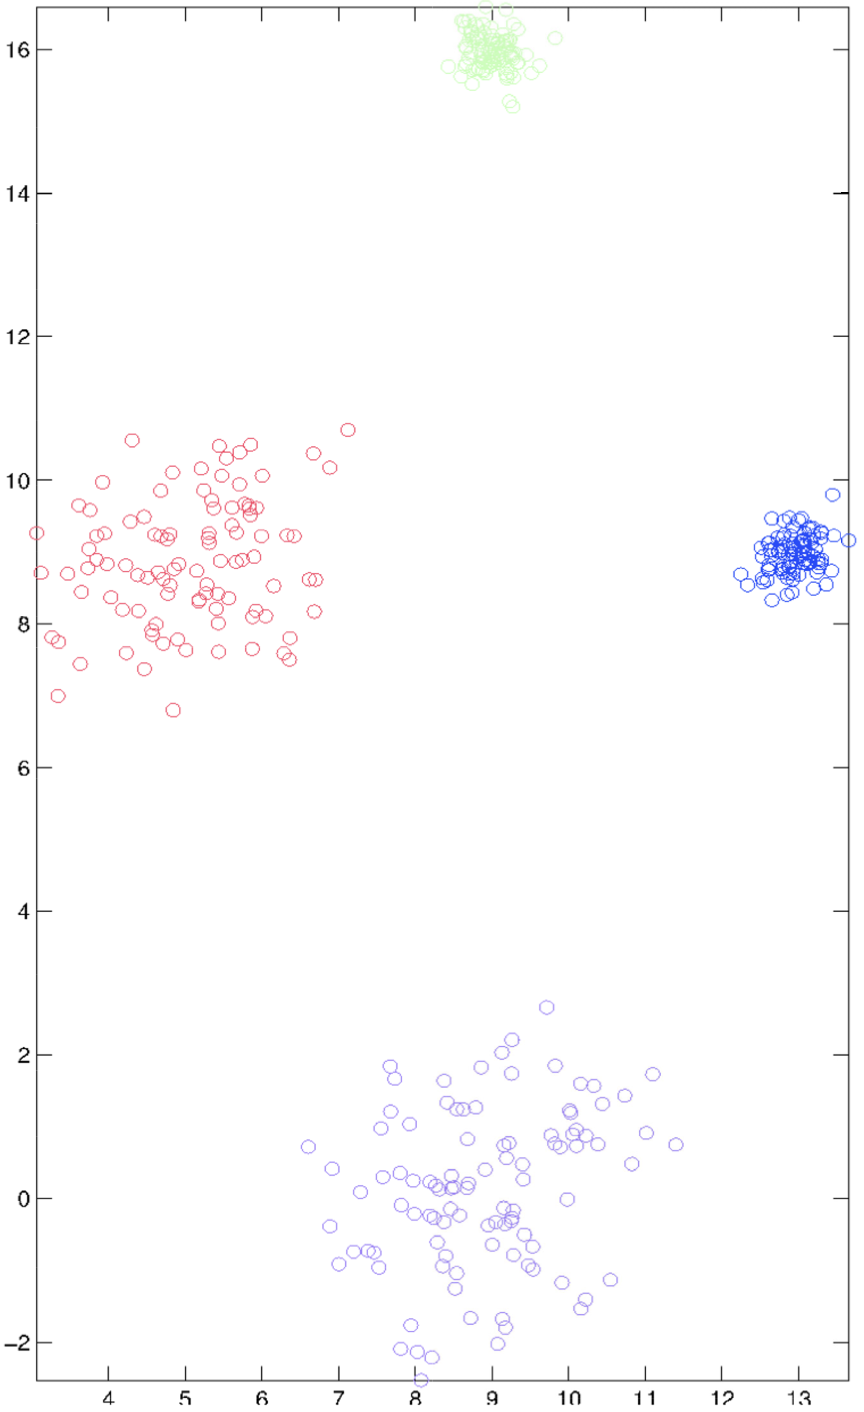
\includegraphics[scale=0.5]{images/Q2P4E.png}
\end{center}

\begin{center}
    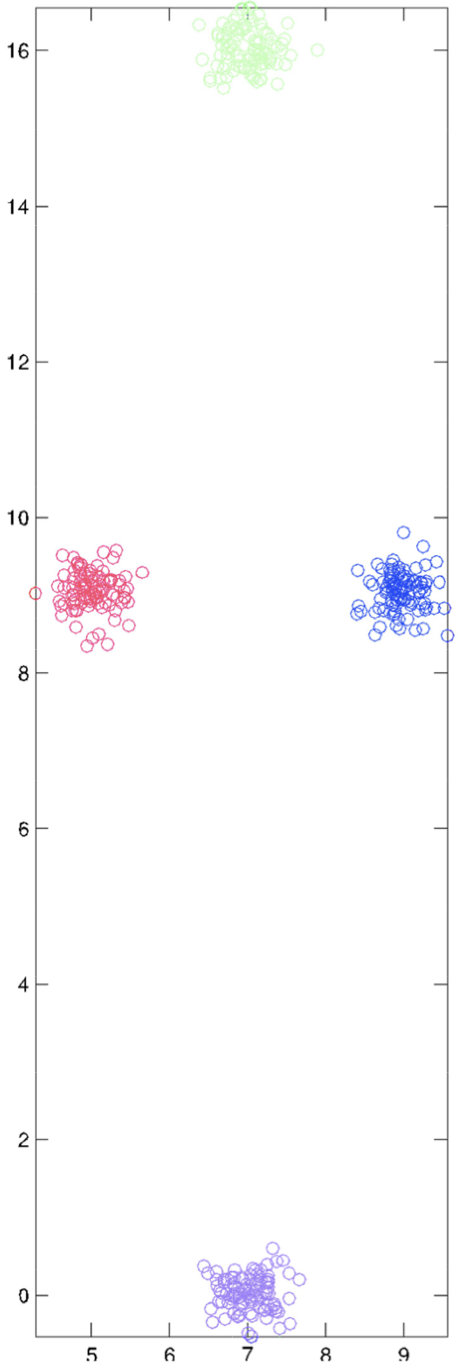
\includegraphics[scale=0.5]{images/Q2P4F.png}
\end{center}

\section{Neural Network}

\subsection{}
You are given the following neural networks which take two binary valued inputs $x_1,x_2 \in \{0,1\}$ and the activation function is the threshold function ($h(x) = 1$ if $x > 0$; $0$ otherwise). Which of the following logical functions does it compute, OR, AND, NAND\@? Please provide your argument.

\begin{center}
    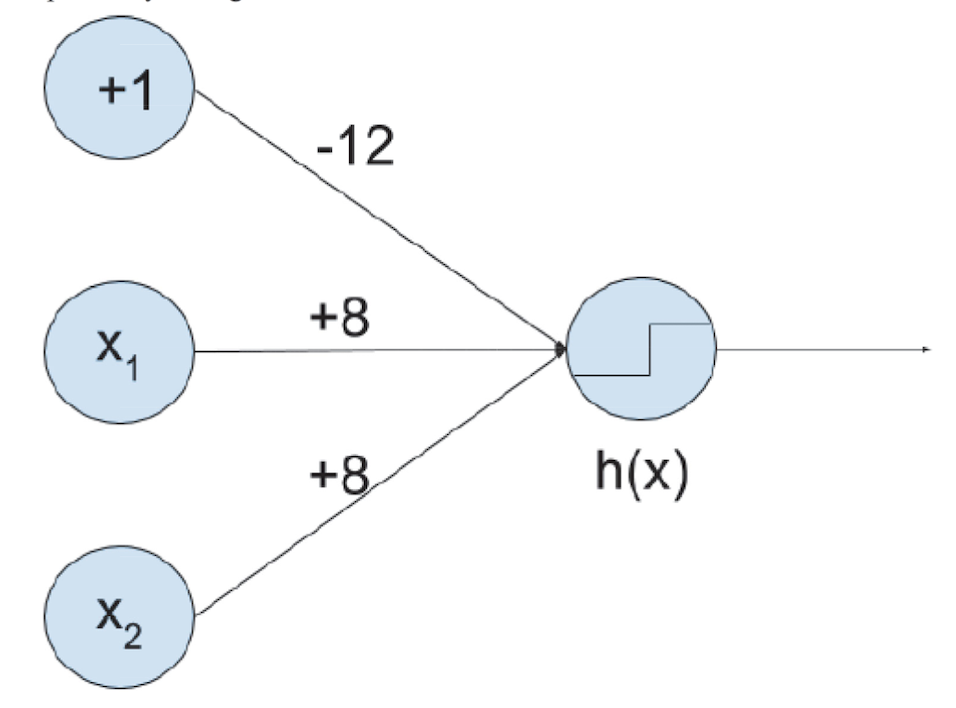
\includegraphics[scale=0.5]{images/Q3P1A.png}
\end{center}

\subsubsection*{Answer:}
This is a AND function due to $x_1$ and $x_2$ both being 1 or true would result in the output being greater than 0. Vice versa, if either $x_1$ or $x_2$ is 0 or false, the output would be less than 0 and the result of the network would be 0.

\subsection{}
We have a function which takes a two-dimensional input $x = (x_1,x_2)$ and has two parameters $w = (w_1,w_2)$ given by
\begin{equation}
    f(x;w) = {\sigma}({\sigma}{(x_1w_1)}\cdot{w_2}+{x_2})
\end{equation}
where $\sigma(x) = \frac{1}{1+e^{-x}}$.
We use backpropagation to estimate the right parameter values. We start by setting both the parameters to be 0. Assume that we are given a training point $x_1 = 2, x_2 = 0, y = 5$. Given above information, please find the value of $\frac{\partial f}{\partial w_2}$ based on the chain rule.

\subsubsection*{Answer:}
\begin{equation*}
    \frac{\partial\sigma(x)}{\partial x} = \sigma(x)(1-\sigma(x))
\end{equation*}
\begin{equation*}
    \frac{\partial(\sigma(x_1w_1)\cdot w_2 + x_2)}{\partial w_2} = \sigma(x_1w_1)
\end{equation*}
\begin{equation*}
    \frac{\partial f}{\partial w_2} = (\sigma(\sigma(x_1w_1)\cdot w_2 + x_2)(1-\sigma(\sigma(x_1w_1))\cdot w_2 + x_2))\cdot\sigma(x_1w_1)
\end{equation*}
$x = (2,0)$, $w = (0,0)$
\begin{equation*}
    \frac{\partial f}{\partial w_2} = (\sigma(\sigma(2\cdot0)\cdot0 + 0)(1-\sigma(\sigma(2\cdot0))\cdot0 + 0))\cdot\sigma(2\cdot0) = 0.25
\end{equation*}
\end{document}